\chapter{Replay-driven Fault Navigation}
\label{cha:solution-design}

With Replay-driven Fault Navigation, we address four challenges when
debugging distributed applications: observing and logging failures,
classifying and connecting logs, reproducing failures, and associating
server events with code locations. More specifically, our approach
consists of the following four steps:

\begin{enumerate}
\item We employ a lightweight record or logging mechanism on each
  server, to collect information about communication in the
  network. We combine the separate logs into one, by means of partial
  ordering using Lamport clocks~\cite{lamport1978time}. This step
  provides an improvement over the heterogeneous and unordered logs
  developers have to deal with today.
\item We identify failing and passing runs among logged events by
  connecting assertion failures in the execution with observed network
  traffic. We compare failures and passes to infer critical regions in
  the systems' communication patterns. Using this information,
  developers can focus on the relevant sections of the logs.
\item We use recorded communication as patterns to replay failing
  network schedules and check the replays for assertion failures. If
  the defect is related to a network scheduling problem, the failure
  will reproduce reliably. In that case, developers gain confidence
  that the failure is indeed caused by variance in the network
  communication schedules. Additionally, developers gain a means to
  reliably reproduce the failure for further debugging.
\item Finally, we use failure replay for debugging. We refine recorded
  data during replay to associate network events with code
  locations. We present both in a tool that allows developers to move
  between the two abstractions freely~\cite{Stanley2009}. This way,
  developers can inspect network events presumably corresponding to
  infected state at the program code level, an use additional replays
  to inspect execution state at this point.
\end{enumerate}

\section{Live System Observation}
\label{sec:lightweight-tracing}

In order to understand a bug, developers iterate over the same code
paths, inspecting different aspects of the program state. In order to
do so, they need some notion of logical event order, to infer causal
relations between events. In \autoref{sec:observation-logging}, we
also argued that it is important to have data from the live system to
debug distributed applications, because only the live system may
exhibit the specific timing behavior to produce a sporadic bug.

\subsection{Logical Communication Schedules}
\label{sec:logical-schedules}

Communication schedules in distributed systems can only be established
for subsets of all gathered network events, because communication
between servers in a distributed system is truly parallel, and some
events may thus happen at the same time, or so close in time as to
have no effect on one another. To understand causes and effects in a
distributed system, we have to establish the order of events in the
communication.

Network communication events occur at different levels of abstraction,
corresponding to layers of the \ac{osi}
model~\cite{zimmermann1980osi}. We chose to establish schedules at the
\emph{application layer} of the \ac{osi} stack, so they may be easily
correlated to the code that created them.  Previous work has mostly
focused on recording events on the \emph{transport layer},
i.e. \ac{tcp} and \ac{udp}
events~\cite{Geels2006Replay,Konuru2000}. However, network and Web
development frameworks usually work at the application layer, sending,
for example, \ac{http} requests or \textsc{sql} queries. These
high-level events may correspond to multiple events on the transport
layer. These transport events have little meaning for a developer
working on the application layer, but combining the transport events
back into application layer events is very difficult in a user space
library that does not have access to \eg \ac{tcp} sequence
numbers. Recoding schedules at the application layer allows us to
provide a user-space solution at a, for developers, meaningful level
of abstraction.

\subsubsection{Partial Ordering of Events}
\label{sec:lamport-clocks-1}

In most systems, the order in which events occur is fundamentally
important to our way of reasoning~\cite{lamport1978time}. We say that
event A happened at 3:15 if it happened \emph{after} our clock read
3:15 and \emph{before} it read 3:16. We call this order the
\emph{logical schedule}~\cite{Konuru2000} in which the events
occurred. The actual timing information (whether the event happened
\emph{at} 3:15, or between 1 and 59 seconds later), the \emph{physical
  schedule}, is only a more specific representation of that ordering.

However, for systems capable of parallel execution, such as the
distributed systems, a universal before relationship is not easily
obtainable and may not physically exist. To solve this problem,
logical, or \emph{Lamport} clocks~\cite{lamport1978time} are used to
establish a partial ordering. Lamport clocks provide a logical
schedule that can be implemented in a parallel system. Central to
logical schedules is the causality between events. If we know that an
event A triggered an event B, we know that A must have happened before
B, even in the absence of a clock.

The original implementation idea by Lamport, also implemented in this
work, is still widely
used~\cite{Konuru2000,Stanley2009,Geels2006Replay,altekar2009odr} and
extension such as Vector Clocks~\cite{Mattern1988}, Version
Vectors~\cite{Parker1983}, and Interval Tree Clocks~\cite{Paulo} exist
for more specific scenarios.

\subsection{Continuous Logging}
\label{sec:continuous-logging}

The traditional stop-the-world debugging approach is ill-suited for a
live system that only exhibits the erroneous behavior sporadically. We
have argued in \autoref{sec:conn-serv-code} that developers cannot
stop processes on different machines at the same time. First, this is
technically impossible, because there is no way to perfectly
synchronize all processes. Second, it is also impractical, as stopping
the live system will make it unavailable for users.

Other debugging approaches observe the live system and gather enough
data to allow inspection of the relevant program state at a later
time. One approach is to log all execution state~\cite{Stanley2009},
so developers can inspect that information offline at a later
time. However, such logging imposes a significant overhead, which
makes this approach unsuitable for continuous logging in the live
system. Other approaches~\cite{Konuru2000,Geels2006Replay} have shown
that it is possible to record just enough information to guide the
system down the right path during subsequent executions. These latter
approaches have little overhead and are suited for continuous logging.

We assume that each server in the network is in itself deterministic,
and that any non-determinism is introduced by access-races to shared
resources, i.e. the network and other servers. If each node is indeed
deterministic, that means that if network requests arrive in the same
order, the same \emph{class} of output---correct or incorrect---is
produced. Furthermore, we assume that nodes and the network are
well-behaved, meaning, that nodes do not suddenly change their
\textsc{IP} addresses, and network segments do not suddenly disappear,
making nodes unreachable. We realize that this may preclude usage of
our approach for less dependable networks.

This means we only have to record the order and type of \ac{http}
requests between any two communication partners to faithfully
reproduce communication, applying only traffic shaping. Compared to
recording the request contents or partial execution traces, this is
little information, with little space
overhead. Indeed,~\cite{Geels2006Replay} has shown that the necessary
information overhead encoded into the request packages may be as
little as adding an 8 byte Lamport clock. Since we do not store the
message contents, these 8 byte plus identifiers for the two
communication partners are all our storage requirements for network
events at runtime. As identifiers, \textsc{IP} addresses and port
numbers may suffice, adding 4 byte for the port and 16 byte for the
address, in the case of \textsc{IPv6} addressing. For an application
that keeps the last 1,000,000 requests stored in its logs before
rotation, this costs about 26 MiB in storage space.

Adding logging to an existing application will change its execution
behavior. The additional execution steps impact performance and thus
timing and memory behavior. Even slight changes can have a large
impact if they increase the likelihood of, for example, cache misses
in the \textsc{CPU}.

Nevertheless, choosing a lightweight logging mechanism is worthwhile
to minimize disturbance. Furthermore, by enabling the logging facility
in the deployed system, the overhead of logging is no longer a
sporadic disturbance that only occurs when running a system
diagnosis. Instead, the disturbed behavior becomes the normal
behavior.

Minimizing disturbance for debugging is particularly useful for
non-deterministic failures, but is a generally desirable property of
debuggers. It minimizes the potential for failures that occur only
during debugging, so-called \emph{Heisenbugs}.

\subsection{Mixed Environments}
\label{sec:mixed-environments}

With continuous logging in a distributed system one has to consider
organizational and practical boundaries. To introduce generalized
logging into a distributed system we need to extend services on
different nodes. Not all these nodes are under developer control, or
have source code readily available to extend them. Our tool thus has
to function in a mixed environment. For \ac{http} communication, this
is easily possible by adding custom headers, which will be ignored by
non-logging clients. We do not regard lower levels of
communication. Ways to deal with services at the transport level have
been covered in other work~\cite{Geels2006Replay,Konuru2000}.

Servers that are part of our distributed system, in the sense that
communication with them contributes to the purpose of the system, can
be either cooperating or non-cooperating. During normal execution,
non-cooperating servers simply ignore the additional headers for
Lamport clocks. To combine the logs at a later time, any discovery
mechanism, from a well-known port to ZeroConf\footnote{ZeroConf
  Internet Engineering Task Force (IETF) Internet Draft\\
  \url{http://www.watersprings.org/pub/id/draft-ietf-zeroconf-reqts-12.txt}\\
  accessed July 21, 2012} can be used.  Incoming and outgoing events
for sent and received requests, respectively, can then be added for
non-cooperating servers by means of inference.

This will necessarily create incomplete logs in the presence of
non-cooperating servers, but this can be safely ignored if no state is
shared with other, third-party, distributed systems accessing the same
non-cooperating servers. These systems are common in practice, because
\ac{rest} and \ac{soa} encourage cooperating systems without shared
state. However, this also means that our approach is not well suited
for shared, "cloud" database services and other stateful systems.

\section{Communication Analysis}
\label{sec:comm-constr-analys}

In Replay-driven Fault Navigation, recording communication events
provides data from the live system. Continuous logging will capture
correct and anomalous communication events. Developers need to
understand the difference, why one particular log ends with a failure,
where another ends without one. There is little tool support to find
such variances in server logs, consequently, this is the next step in
our approach.

\subsection{Differencing between Schedules}
\label{sec:diff-betw-call}

To create a tool to find variances in communication schedules, we need
a model of such schedules. We argued in \autoref{sec:requ-based-distr}
that sequence diagrams are well suited to both model network
communication as well message passing between objects. Consequently,
network schedules also form a \emph{call tree}, with requests and
responses representing message sends and returns.

However, network events occur at the higher abstraction level than
message exchange between objects, and differences to single-threaded
objects. In distributed systems, a single server serves more than one
request in parallel, using event loops or multi-threading to process
and send out responses as they become ready. Thus, we cannot assume a
causal relationship between two requests arriving at a server one
after another, and not between two responses leaving the server. The
temporal relationship alone does not imply a causal relationship.

For non-deterministic failures caused by network schedules, however,
we know that variances in the order of events influence one
another. We can use our a diagnosis script to create multiple
schedules that all yield the same result, but vary slightly. Comparing
these schedules, we can find possible causal relationships between
events. For sub-sequences of events that vary frequently across
executions, these events can be assumed to have little or no influence
on one another. Sub-sequences that vary only rarely or not at all are
indicative of causal relations between those events.

Consider our flight meta-crawler bug report in
\autoref{sec:motivating-example}. We can assume that the discrepancy
between the price displayed before and after reservation is due to a
data race between another user reserving a seat on the same plane, and
the user filing the bug report. If we run a system diagnosis it may
pick up a number of users using the system, leading to activity as in
\autoref{fig:flyhehe-pre-booking}. Users booking other airlines prior
to the diagnosis may reserve other flights without causing the
diagnosis to fail. A variance in the reservations prior to the actual
diagnosis---in the shaded area---is thus inconsequential to the result
of the diagnosis. Only variations in the order of clients booking the
same flight as tested in our diagnosis script have an impact on the
result.

\begin{figure}
  \centering
  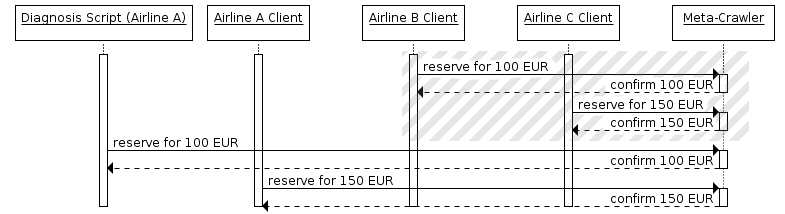
\includegraphics[width=\linewidth]{flyhehe-pass-pre-variation}
  \caption{Activity Prior To Successful Diagnosis}
  \label{fig:flyhehe-pre-booking}
\end{figure}

\subsection{Associating Variations and Assertions}
\label{sec:assoc-vari-with}

The diagnosis script is useful not only for producing similar
schedules, it also includes assertions that test the outcome of the
tested behavior. If the diagnosis reproduces a bug, those assertions
will fail.

Variances between passing and failing schedules can be used to reduce
the entry points that need to be checked for defects. If we compare
all passing schedules, we find variances that probably have no bearing
on the outcome of the test. If we compare them against the failing
schedules, and subtract the variances within the passes themselves, we
may find sequences that vary only between the passing and the failing
schedules. Those may be of particular interest to the developer,
because they are likely to be related to the failure. Such a variance
can occur in the unshaded activity in
\autoref{fig:flyhehe-pre-booking}. If the second reservation for
Airline A were sent prior to the receipt of the confirmation in the
diagnosis script, a critical race may ensue that causes the diagnosis
to fail.

Failing schedules have variances within themselves. We use this to
heuristically mark these variances as less likely causes than others,
as these variances then seem to have no impact on the outcome, since
they all produce the failure. Variances within the failure schedules
that also vary against all of the passing schedules are more likely to
be only on the path of the infected state of the program, not the
cause of the defect itself.

Consider \autoref{fig:flyhehe-failing-variation}, as an example for
variances in failing schedules. The failures, as the passes, may vary
in the order of reservations prior to the actual diagnosed
reservation---the shaded area near the top. However, the failures may
vary also in the order of the requests and confirmations for
reservations made by the diagnosis and the Airline A client---the
crossed area below. The only passing schedule for that part of the
communication is the one we see in
\autoref{fig:flyhehe-pre-booking}. Thus, the initial variances within
the failing schedule that also occur in the passes are of little
interest to the developer and need not be considered. The variances
near the end of the schedule, however, that are only between failing
schedules and do not vary within the passes can be considered likely
causes for the failure. We need to guide developers towards that part
of the communication for further debugging.

\begin{figure}
  \centering
  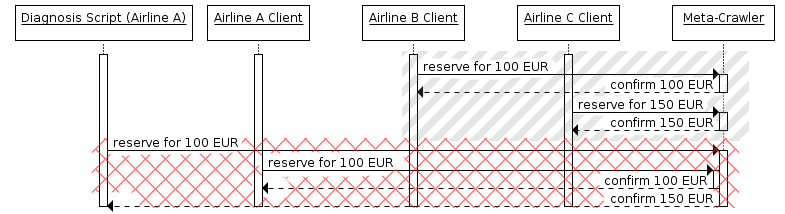
\includegraphics[width=\linewidth]{flyhehe-pass-failing-variation}
  \caption{Variations Failing Diagnosis Runs}
  \label{fig:flyhehe-failing-variation}
\end{figure}

% We could consider the interesting regions to be critical regions in
% the communication schedule, where even slight variations may cause a
% failure, and the variations that occur within passes as well can be
% considered forgiving regions of communication, where variance has
% little or no impact on the successful execution.

Finally events that occur late in the schedule are less likely to be
the original cause of a failure. To express this in our heuristic, we
adjust the probabilities linearly with respect to the sequence number
of the event within the schedule.

\section{Replay and Reordering}
\label{sec:comm-repl-reord}

Up to this point we have been inspecting the system without knowing
whether varying communication schedules are the cause for a
non-deterministic failure. We can now reinforce this assumption by
running failing schedules multiple times through what we call our
\emph{re-ordering replay scheduler}. The scheduler enforces a
particular order in network communication traces, which means we can
replay a failing trace multiple times with exactly the same order of
network events. If the result is consistently the same, even if the
failure occurred only sporadically before, we have a strong case to
believe that it was caused by this particular schedule, and further
inquiry with our method is warranted.

In some cases the outcome may vary even if our scheduler enforces a
failure schedule. An example is an improper implementation of
timestamp parsing on one machine, that causes the bug whenever the
timestamp has one of a few particular value. Such a bug will occur
regardless of the network schedule, and our approach is not suitable
to debug these kinds of failures. However, even in that case the
developer will have learned that non-determinism in the network
schedules is not responsible for the failure, and can focus his
debugging efforts on each server in turn, using traditional debugging
approaches.

\subsection{Re-ordering Scheduler}
\label{sec:re-order-sched}

The scheduler itself works as an intermediate layer between the
application code and the network, and effectively acts as a traffic
shaper\footnote{Internet standard definition of ``Shaper'' in RFC
  2475\\
  \url{http://tools.ietf.org/html/rfc2475\#section-2.3.3.3}\\
  accessed July 25, 2012}. It tries to re-order access to the shared
resource---the network---to enforce a particular, prerecorded
schedule. This is done by holding and releasing incoming and outgoing
communication according to the schedule, rather than the order in
which they arrive.

Since we want to record application layer events, it is most natural
to insert the scheduler between the application framework code
responsible for sending and receiving, and the underlying language or
operating system primitives. This has the additional advantage that
the scheduler can be programmed with some knowledge about the
framework, and thus the ability to communicate its actions to the
developer on the level of abstraction of the framework. This not only
keeps the developer in control of the debugging process, it also
allows meaningful configuration of the scheduler heuristics. Because
we record only the partial order and identifiers for communication
partners for events, the scheduler can only replay scheduled events
that occur in the system at the time of re-scheduling. That means that
\emph{all} servers that were active during record must be active
during replay as well. This may not always be the case, and scheduling
on the application layer allows us to communicate conditions for
holding and releasing events to the developers, so they can take
appropriate action, such as choosing another schedule or ensuring the
required servers are indeed online.

As an example, the scheduler can to re-order according to a schedule
that includes communication with a backup server. This backup server
may only be active at particular times of the day, say, at
night. Developers debugging a problem during the day may cause the
scheduler to wait for a long time---up until the backup server is
active. The system will seem to hang. Being able to communicate to the
developers the reason for waiting helps them to understand the
possible cause of the failure, and either bring the backup server
online for the purposes of debugging, or choose a schedule recorded at
another time.

Generally, such a scheduler has to control all points in a given
framework where application layer requests are received and
released. A possible algorithm for such a scheduler is given in
\autoref{fig:reorder-sched}. Such a scheduler will have to distinguish
whether the framework is using multiple threads of execution or just
one.

For our assumption of determinism on each server to hold,
multi-threaded servers need to be synchronized on send and receive
events, by using some kind of synchronization mechanism such as, for
example, semaphores. When a request is received, the scheduler checks
whether all requests that are expected to arrive before this request
have been received. If they have, the requests can be released into
the framework. Otherwise, the current thread of execution has to be
suspended until all previously scheduled requests have been
received. Upon release of a request into the framework, all threads
waiting on this request can be released, too. Similarly, for sending
responses, the scheduler holds those responses until all previously
scheduled responses have been sent by the framework.

Single threaded servers as they are used, for example, for event
loops, cannot be stopped if a request arrives too early, as that would
prevent any other requests from being processed. In this case, the
scheduler will receive requests into a buffer, and keep receiving
until the currently scheduled requests arrives, which is then
returned. Once the server is ready to process the next request, it may
be released directly from the buffer, if it was previously received,
skipping the network access altogether. In single-threaded mode we can
ignore outgoing requests. Under the assumption that the server works
deterministically, it will send the responses in the correct order if
it receives all requests in the correct order.

\begin{figure}
  \centering
  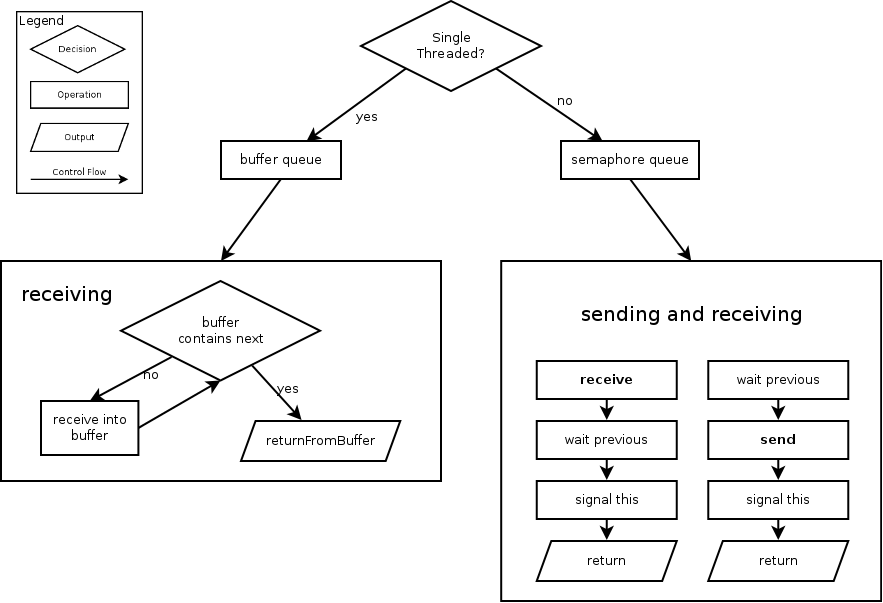
\includegraphics[width=\linewidth]{scheduler-ablaufdiagramm}
  \caption{FlowChart~\cite{Bohm1966} of Re-ordering Scheduler}
  \label{fig:reorder-sched}
\end{figure}

\subsection{Fault Navigation Over Multiple Runs}
\label{sec:replay-driven-fault}

After reproducing a failure, developers have to inspect the program
state. In \autoref{sec:lightweight-tracing} we have argued that a
lightweight logging approach is preferable for observations on the
live system, both to minimize the performance impact and the
possibility for Heisenbugs. However, this approach prohibits recording
information about the program state at this stage.

With the scheduler, however, we can enforce failure schedules as
needed for further analysis. Based on the initial communication log we
can, in a re-run, add an initial, shallow log of the called methods on
each node. This is based on the earlier work about incremental, online
analysis of runtime behavior~\cite{Perscheid2010}. Given the source
code running on the servers, this information can be connected in a
debugging tool to present a call tree to the developers.

While developers explore the call tree, it is interactively refined
on-demand. We add one-shot logging at points of interest as needed,
without disturbing the deployed system unduly. Because the the
scheduler holds on to parallel requests, the schedule will be
consistent with earlier runs and the program state will be a proper
sample.

\subsubsection{Recording the Right Data}
\label{sec:record-right-amount}

In order to assume that the observed program state for a particular
replay is a proper sample for this replay, we have to previously
record sufficient information to decide whether or not a given replay
is really equivalent to an earlier one. This means we may have to run
multiple replays for any given inquiry by the developer. Since we
record only the partial order and communication partners there is some
initial uncertainty about whether the message content is
equivalent.

Before any inquiry, we collect message samples for all communication
in a replay. This diminishes the aforementioned uncertainty, because,
on the application layer, we can treat message contents as parameters
to the remote system. This way, we can not only define a maximum
variance for messages to decide call equivalence, developers can also
review the message contents and decide, depending on the domain,
whether the schedule is correct.

\subsection{Online Replay}
\label{sec:online-replay}

In general our replay and record mechanism works for all the different
environments mentioned in \autoref{sec:observation-logging}, from
local developer setups to the deployed system. We consider the
deployed system to be the superior basis to acquire information during
replay.

A test environment already offers much better control to the
developers for debugging failures, even without the application of
Replay-driven Fault Navigation. Combined with our approach, we could
use the test environment to replace the diagnosis script with a more
"`traditional"' test, i.e a piece of executable code that resets the
test environment to a known state and then replays the recorded
live-system schedule within the test environment. Communication
partners that are part of the deployed, but not the test system have
to be mocked with prerecorded data.

The advantage of this way of using our approach is the amount of
control it offers. If the setup is sufficiently close to the deployed
system, the replay will inject the deployed system behavior into the
test environment. Multiple replays may be executed in quick
succession, as network and processing delays are small due to the
close physical proximity of servers in the test environment, and the
reduced load without live users that the system has to process, too.
Yet, those same variables may cause the test environment to produce
rare, non-deterministic failures at a different rate, or not at
all. Additionally, mocking servers that are not part of the test
environment introduces another uncertainty into the system, which
cannot be trivially proven to have no impact on the failure. Thus, we
focus on applying the replay mechanism directly to the deployed
systems.

\subsubsection{Distributed Recording}
\label{sec:distr-repl-reord}
\label{sec:distributed-scheduling}

Running debugger processes across a network and controlling them from
a developer machine introduces delays that prevent synchronous halt,
step, and resume. We circumvent these delays by using on-demand
scheduling and recording, yet, the question remains how to propagate
on-demand record in a synchronized manner in the distributed
system. We have not implemented such a mechanism, but different
designs come to mind, for the open-world case and the closed-world
case, respectively.

Our scheduler can be used to instrument some or all of the servers in
the deployed system, to replay schedules in the same environment in
which they were recorded. The advantage of this approach is the
availability of live data and more faithful reproduction of the
failure. It is non-trivial to reproduce the setup and state of a
sufficiently complex distributed system in a local test
environment. It may be easier to replay in the deployed system than to
re-create the deployment correctly enough to obtain the same execution
behavior.

In order to recover more data from the live system during replay than
we already have, the scheduler needs a mechanism specify recording
on-demand. This means that, while the developer is debugging, the
diagnosis script and scheduler replay the debugged schedule again and
again, each time recovering one more piece of information, like for
example a call stack, values of variables, and so on. Recovering only
one piece at a time means that developers have to wait until the
script has been re-executed and the information was recovered, but it
ensures minimal disruption to the service of the deployed system. This
impedes the fidelity of the approach outlined in approaches such as
the Path Tools~\cite{Perscheid2010}, which we build upon, but we show
that effective debugging is still possible with this approach
(\cf{\autoref{sec:wrapper-latency}}).

As mentioned above, our scheduler only works for well-behaved clients
in a functioning network, and in the absence of those, heuristics need
to be applied to ensure continued availability of the distributed
system overall. Since the scheduler cannot do more than wait for the
appropriate messages to appear to shape the traffic into the right
order, it depends entirely on network connectivity and deterministic
clients to reproduce a schedule. These constraints are not always met,
as network and server outages may make crucial parts of the schedule
temporarily unavailable. In this case, the scheduler will begin to
hold requests and responses on all nodes until temporary outage is
over. This is not desirable, as it effectively shuts the distributed
system down. We think that configurable heuristics for timeouts,
dropping requests or patterns for requests that should never be
rescheduled can circumvent this problem.

\paragraph{Closed-World Case}
\label{sec:clos-world-case}

In the closed-world case, all the servers in our distributed system
use our scheduler, and we have full control over the in- and output of
the system, both during record and replay. Also, no servers are added
or removed between record and replay.

During recording, each server generates a \ac{uuid} for itself, from
any suitable source such as the \textsc{mac} address of the network
card or the \ac{uuid} of other hardware components such as hard
disks. After the first execution, the log files from different servers
are aggregated into one and their \acp{uuid} are mapped to their
recorded \textsc{IP} addresses. Thus, the server \ac{uuid} allows us
to associate a server uniquely with events in the schedule.

During replay, the desired schedule is chosen at the developer
machine. The additionally desired information is added in form of
queries to the appropriate schedule event. For example, at the
beginning of a debugging session with a particular schedule, we
re-execute the schedule and for each event record the first few
hundred bytes of data sent or received. The schedule is split into
parts for each server that contributed to the original schedule and
sent out to those servers, via the same mechanism used to aggregate
the logs (\cf{\autoref{sec:mixed-environments}}). On each server the
scheduler will then read the log and re-order network access to suit
its partial schedule. Whenever an event with an additional query is
encountered, the scheduler will execute the query and log the result
before continuing its operations. At the end of each re-execution logs
are again aggregated from all participating servers and presented in
the debugger.

\paragraph{Open-World Case}
\label{sec:open-world-case}

In the open-world or mixed-world case, not all participating servers
include our scheduler or allow us to record at will---it may be
desirable, for example for Web services, to offer only replay data,
but not source code, to their developers. In the open-world case we
can also allow the number servers to change between record and replay.

In this case we record all message contents between scheduled and
non-scheduled servers. During the replay phase, any network event from
a non-scheduled to a scheduled server is performed with the recorded
data, not with the real network. The wrapped framework call for
network access is not executed. Likewise, any message sent to a
non-scheduled server during the record phase need not be sent again
during replay.

\subsubsection{Configuration Options}
\label{sec:required-heuristics}

For well-behaved clients in a closed-world setup the scheduler will be
able to perform its operation without problems, because given we start
with the right network event, all required events will eventually be
generated and the scheduler on each server can re-order events as
necessary. However, in the mixed-world case, with non-scheduled
servers, or in the face of unreliable network, with servers that
appear or disappear between record and replay---think of Web page
clients that use the deployed system while record and replay are in
progress---developers have to configure the scheduler to work under
these circumstances.

A scheduled server may receive events from servers that are not part
of the schedule, or wait to receive events from servers that were
available during record, but are not anymore during replay. We believe
this problem cannot be solved in a general way, and for these cases we
offer several settings with which developers can configure behavior
for these cases on each server.

\begin{description}
\item[Timeouts] Waiting for events may hold requests and responses
  unduly. A server that keeps no state between requests does not need
  to follow a schedule precisely for the re-execution to be
  useful. For example, in our flight reservation service, the Web page
  server has no state, as all the state is in the cache and airline
  databases. It may be useful to release network events after a
  configurable amount of time, regardless of their place in the
  schedule.
\item[Unscheduled Events] Non-scheduled servers may send events during
  replay that did not occur during record. If dropping these events is
  an option, it may be desirable to do so in order to keep the
  schedule. Otherwise, bypassing the schedule for these events may
  also work, depending on the setup---in our example clients that
  access the flight search during replay can bypass the schedule, as
  the search has no bearing on the reservation bug.
\item[Disruptions] It may be desirable to specify a separate timeout
  to wait for scheduled events. In our example the cache, which is
  queried for searches as well as rates and reservations, should not
  wait too long for an event. If a scheduled event is not generated in
  the network in time, the schedule should be marked as disrupted,
  re-scheduling is aborted, and all pending events are released. In
  this case the re-execution fails and has to be restarted.
\item[Message Level] Developers know their deployment setup best. If
  the re-execution is delayed, because the scheduler is waiting for a
  specific event to be generated from a specific server, this
  information may in itself be useful to the developers, even if the
  event never is generated. For example, if a backup is sent to
  another server from our flight cache every day at noon, and this
  caused a failure, replaying the schedule that includes the backup
  upload event can only work around noon, because otherwise the event
  is not generated. Informing the developer about this can be enough
  to provide a clue about the failure, and is preferable to stopping
  all network communication until the next backup network event is
  generated.
\end{description}

\section{Debugging at Different Levels of Granularity}
\label{sec:debugg-at-diff}

We can record and replay network schedules in the deployed system. We
use this mechanism to refining our recorded data during each
replay. The kind of additionally recorded data includes network event
contents, call stacks, method arguments, and return values. Developers
can use this information to associate events at the network
communication level to method activations at code level.

\subsection{Connecting Network Events to Code}
\label{sec:moving-from-network}

To debug asynchronously communicating applications developers need to
move between the different levels of abstraction, from communicating
servers to message sends between objects. They have to map the
observed network behavior to the original intentions expressed in the
code. In our approach we support this mapping with a tool that
integrates a network events with call trees.

One conventional approach to debugging distributed, communicating
applications is to try and determine likely locations of defects in
the code from the communication log, and the use a sequential debugger
to debug each server process independently to figure out which code
segment is responsible for a given unanticipated or erroneous network
event. However, with Web and other applications increasingly utilizing
asynchronous communication and event loops, mapping from code
locations to network events and back is becoming harder. While
outgoing requests can still be identified because they use only a
small number of framework calls for network communication, incoming
communication is increasingly handled by event callbacks. For this
style of communication, a debuggers' stack view will only reach back
as far as the last receive, with no possibility to look back further
to inspect previous communication events.

We propose tool support to provide an integrated view of both network
communication and call tree, synchronized to move freely from code to
network events and back. We argued that debugging across a network of
servers is similar to debugging across threads or communicating
objects. It appears natural to merge the communication trees and view
network communication as nested calls that originate from and return
to code. A debugging tool for distributed debugging may generally
support multiple, synchronized call trees, each call tree may show
network events or communicating objects.

Using our approach, developers are free to move through the recorded
execution both on the network level or on the code level. The
distributed debugger provides two synchronized views, one for the
global view on the network event log, and the other for a call tree
specific to the currently debugged server. Developers may interact
with the network view and, for example through clicking on an event, a
re-execution is triggered. This re-execution adds a query to the
schedule that logs all method activations on the server receiving the
event, in case of a request, or sending the event, in case of a
response. With that information, we can build an execution-specific
call tree for this server, and highlight the method activation that
was responsible for generating or receiving the network event. Since
we have recorded the full call tree, the developer is now free to move
up and down the call tree to orient himself in the code.

The debugging tool can use the information about sender and receiver
for each event to show the code that corresponds to the event. That
means showing the sender code for outgoing events and the receiver
code for incoming events. If the source code for a particular server
is available, the tool can automatically show the method responsible
for each communication event in the call tree. This provides
additional insight to the developers. They can then inspect method
arguments or local values, which will trigger additional re-executions
and recordings as needed, to find out more about how the event data is
generated or processed.

We have decided against adding support to show call trees from
multiple servers side by side, because we think the network event view
is more suitable to navigate from one server's call tree to
another. The interfaces between the different servers are encoded in
the communication data, rather than the arguments or local variables
in the servers' methods, so we think that presenting multiple call
trees side by side has no additional value.

\paragraph{Inferring Interfaces Across Languages}
\label{sec:inferr-interf-across}

A consequence of using our approach is the direct connection our
debugger can draw between code in different languages running on
different servers. Through the network events, we can infer interfaces
between those different languages. Those interfaces are implicitly
defined, in most \ac{rest} applications, or have more explicit
definitions only in another language, for example in \textsc{corba},
\textsc{soap}, or other kinds of middleware.

Without such explicit definitions so-called \ac{rest} interfaces
rarely follow a specific pattern for their communication. Oftentimes,
the wire encoding of choice is \ac{json}, because it is easy to use in
the browser and parser implementations exist for most
languages. However, \ac{json} as a simple key-value format for data
transfer offers no default interface definition language, and various
services\footnote{\xspace\hairspace
  Github API v3: \url{http://developer.github.com/v3/}\\
  Twitter REST API: \url{https://dev.twitter.com/docs/api}\\
  accessed July 25, 2012} offer no more than textual descriptions and
examples for their \ac{rest} \acp{api}. Such descriptions are hard to
verify against an implementation.

The more immediate issue with informal descriptions of \acp{api} is,
however, that outdated information is difficult to update, as this
requires checking the source code and update the documentation with
the informal \ac{api} description. With our approach, the interface
can be determined without access to the source code, by reviewing
recorded message contents for valid communication. If there is a
communication error somewhere in the log, and it is suspected to be
due to improper usage of the \ac{api}, the event's message contents
need only be compared against a log of a working communication, to
test this hypothesis.

Once such an error is discovered, our approach offers the direct
connection from the problematic events to the source code where the
events are generated and received. Thus, developers can test their
hypothesis and move to the appropriate piece of code to fix a
potential problem.

%%% Local Variables: 
%%% mode: latex
%%% TeX-master: "thesis"
%%% End: 
